\documentclass[12pt]{article}
\usepackage[affil-it]{authblk}
\usepackage{verbatim}
\usepackage{graphicx}
\usepackage{float}
\usepackage[utf8]{inputenc}

\title{Analisys of the STCP transport network}
\author{Diogo Bogas}
\affil{DCC/FCUP}
\date{December 12, 2016}


\begin{document}
\pagenumbering{gobble}
\maketitle
\newpage
\pagenumbering{arabic}

\tableofcontents


\section{Abstract}
This theme aims to do an initial analisys of the complex network that represents all the bus lines belonging to STCP. The student will start by creating the network, with automatic data extraction from sources like the website stcp.pt.
Then, with all the gathered data, there should be a preliminary data analisys with focus on node centrality, degree distribution and charateristic patterns.

\section{Introduction}

A network is a catalog of a system\textsc{\char13} s components often called nodes or vertices and the direct interactions between them, called links or edges.
Some good examples of networks, are social networks like Facebook and Twitter.
This article uses networks to represent the services offered by a bus company operating in Porto, with the intent of answering some questions like : how many bus stops are there, which street has the most lines going through it and how many times do i have to change bus so i can go from one side of the network to the other. 
 

\section{Data Gathering and Processing}

\subsection{Data source}
The first decision made in this study wasn't what to study about the network, was to know were to get the data. 
The STCP website is a great place to start, as it has all the information on bus lines and bus stops. So, how do we get the information programatically?
The best way to do it, is to read the answer the server gives the client when a request is made. Luckily, this answer is in form of JSON objects, which are easily parsable.
The information the site gives about bus stops and bus lines is enough for the common user, but we need more. There are some aspects we need to derive if we want to do a complete study on the proposed network. Therefore, every piece of information was locally stored.

\subsection{Data storing}
While reading the information from the server answers, i noticed that each time i wanted to read the data i had to , programatically,connect to the site ,and that took too long to be viable. 

A simple answer was to create two .txt files with the information gathered.

One of the files (AllLines.txt) has all the information about each busline.
Each bus line is represented in a single line by a code, a direction, an integer that tells us the total number of stops in that line, and finally, all the stops that compose said line.

The other file (AllStops.txt) has all the information about all the stops.
Each stop is represented in a single line by a stop code, an address, a zone, a name and a pair of floating point numbers that represent it's geographical location. 

All of this information can be refreshed, as there are methods that do so.\\

There is the need for some structures in which to represent all this data we have, so it can be easily used to answer some of the questions raised above. These were made in the JAVA programming language and are described in the apendix for this report.\\

	In quick fashion, the information was grouped in three ways:\\
	
	The normal way, where the information was read from the text file, put into structures and handled like that.\\
	
	 By streets, where the stops were grouped by street, each street was a node and the trips between streets were the edges.\\
	 
	 And by code, where the streets were grouped by code, in a structure called Spot, and a trip between two Spots was an edge.\\
	
	These are the structures used to simplify this study.\\
	Some files, six to be more precise, were not included in this subsection, as they were generated with JAVA to be used by gephi.
	These files are described in the apendix, the generating methods come in the next subsection.

\subsection{Data processing and input creation}
	
	As mentioned before, Gephi was used to study the network. Gephi is a preety powerfull tool, but it requires some form of input. In this particular case .csv files. This subsection describes the methods that process the data (stored in any way described in the previous subsection) and generate the input gephi needs.\\
	Still on the previous subsection, it was mentioned that there were 6 files left to describe. Three of these are groups of nodes, and the other three, groups of edges.\\
	
	The method that creates the .csv file for ungrouped Stops reads the  AllStops.txt file and works from there. In the first line it prints Id;Address;Zone\\;Name;Longitude;Latitude, and then, for each Stop it reads, prints the attributes in the desired order.\\
	For the edges, something similar is done, but now, the data comes from a method that reads the AllLines.txt file and returns us all the edges in an HashMap. Each edge had represented it's source, target, type and weight.
	
	
	
	
\section{Results}
	This first image is the very first piece of information that our tool gave us, a visual representation of all 2416 stops in the network(not using any type of grouping), colored by zone.\\

\begin{figure}[H]
	\centering
	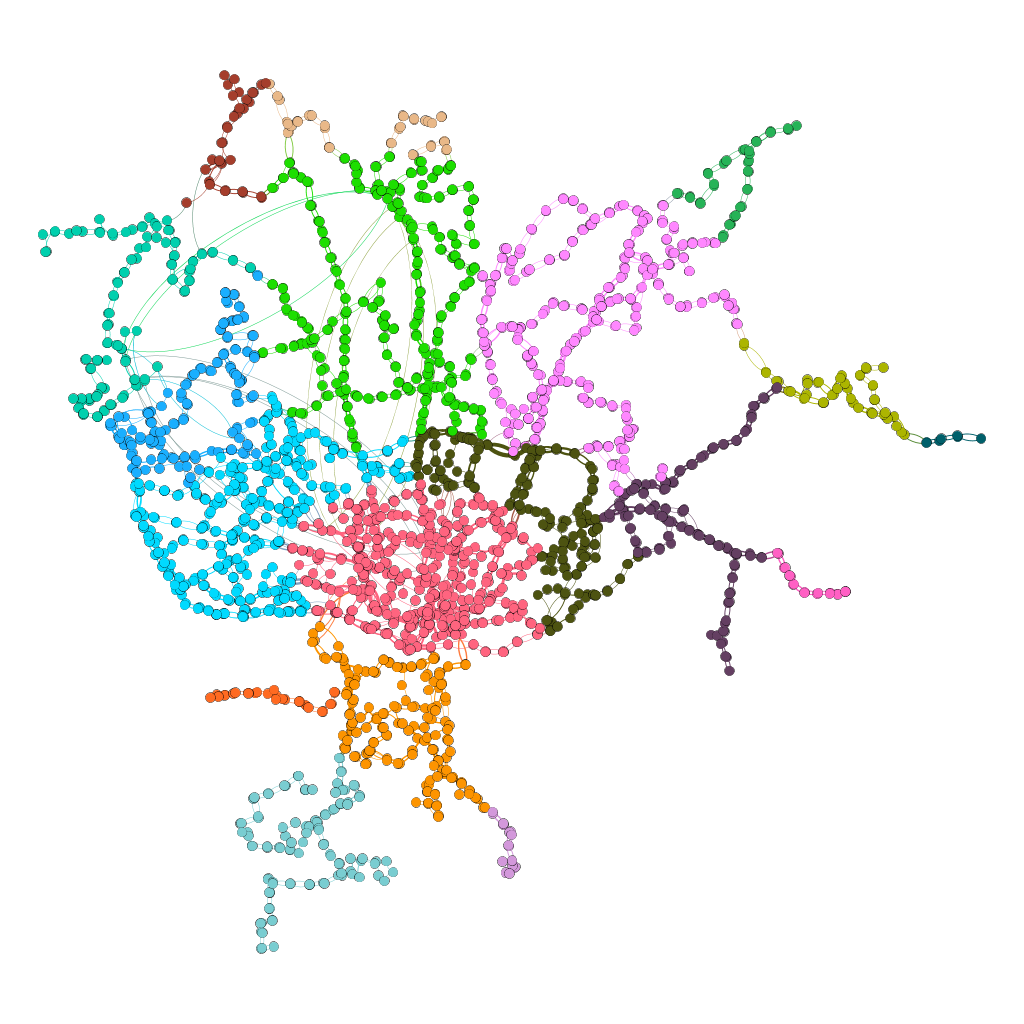
\includegraphics[scale=0.2]{simple_network}
	\caption{The network, without grouping, with stops colored by zones and shown according to geographical coordinates}
\end{figure}
\newpage
The following image is the pallete used to color the network shown above, and it ends up giving us how large is each zone relatively to it.\\
\begin{figure}[H]
	\centering
	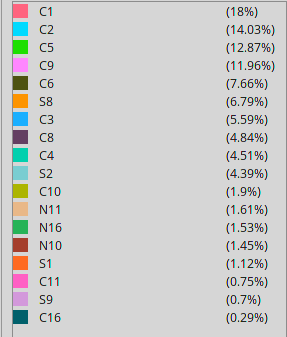
\includegraphics[scale=0.5]{legenda_simples}
	\caption{A table with all the zones, sorted according to size,displaying each zone's color}
\end{figure}

The second question raised in the Introduction section of this report was "Which Stop has the most lines going through it and how many times?". For this, it's better to group the stops by code, and answer a diferent question : "Which Spot has the most lines going through it?", as a Spot is much more influential than a simple Stop. Te answer to this, is in the table below,extracted from spotNodes.csv were the 5 most populated Spots are represented:

\begin{table}[h]
\centering
\begin{tabular}{lll}
Id  & totalStops & linesServed \\
TRD & 6          & 21          \\
BCM & 5          & 20          \\
BS  & 8          & 18          \\
AAL & 6          & 17          \\
CMO & 4          & 17         
\end{tabular}
\end{table}

Checking the Id's in the AllStops.txt file, we get, by ascending order:
Carmo,Aliados,Bom Sucesso,Casa da Música in Boavista and Trindade topping the list.

Analising the nodes, with help from Gephi, we now look to the betweeness centrality. Betweeness measures how many times a given stop acts as a bridge in the shortest path between two other nodes. The next table shows, the "top 10" realative to betweeness:

\begin{table}[h]
\centering
\begin{tabular}{lll}
Nome 		 				&& Zona && Betweeness\\
TRINDADE	 				&&	C1  && 1145449.8813840807\\			
GRACIOSA  	 				&&	C1	&& 771297.5117531752\\		
BOAVISTA CEMITÉRIO 			&&	C1	&& 754319.6087318071\\				
MOREIRA SÁ					&&  C1 	&& 736031.847507471\\		
ASPRELA 					&&	C6	&& 678387.0286322387\\	
AV.ALIADOS 					&&	C1	&& 644478.7719011271\\
TRINDADE 					&&  C1	&& 612273.6268018036\\
IPO (CIRCUNVAL.) 			&&  C6 	&& 611095.6146827459\\
AREOSA 						&&  C6 	&& 601167.8506726616\\
BOAVISTA-CASA DA MÚSICA		&& 	C1	&& 583327.9338578992 	
\end{tabular}
\end{table}

There is a very noticeable pattern, most of the Stops shown above, belong to C1 zone, the center of the network.

\section{Conclusion}
	The results that we obtained colide with the reality.It was expected that the centre of Porto was the most busy zone of the entire network, and proof of that, is that C1 is the biggest zone,and most of it's Stops have the biggest Betweeness in the entire graph. The prior knowledge i had about the service this company provides, and the city itself, helped me as a "sanity check" as the data was processed. This study also allowed me to get a deeper understanding of Graph theory , and it's applications in real life situations.
\section{References}

network definition:
Albert-László Barabasi, Network Science.

circunvalaçao:
https://pt.wikipedia.org/wiki/EN12	

Structure used to facilitate this study:
apendix.pdf
			
\end{document}